\section{Compiler}\label{sec:compiler}

\subsection{Architektur}

\todo{
Visitor Pattern~\cite{gof-design-patterns}.
Dragon Book~\cite{dragonbook}.
}

\begin{figure}
	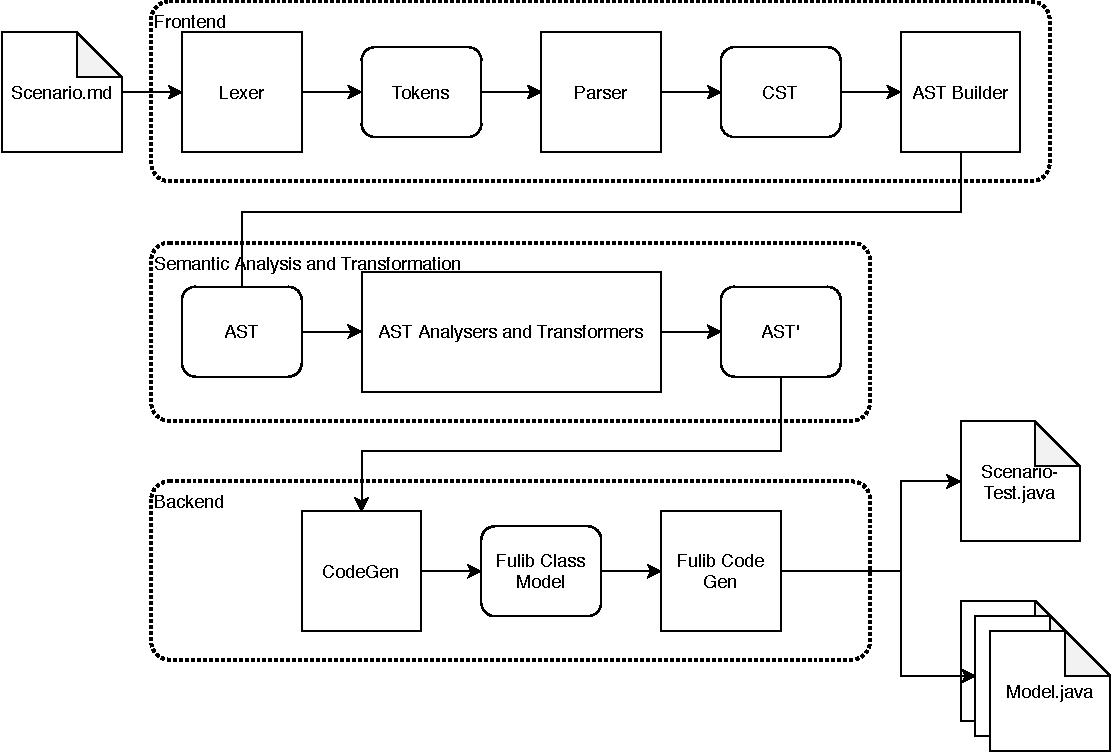
\includegraphics[width=\textwidth]{chapter/fulib-scenarios/img/architecture.pdf}
	\caption{Compiler-Architektur}
	\label{fig:compiler-architecture}
\end{figure}

\subsection{Frontend - ANTLR v4}\label{subsec:frontend-antlr4}

\todo{
Warum ANTLR4 sehr gut für die Sprachstruktur geeignet ist~\cite{adaptive-ll-star,antlr4-reference}.
}

\subsection{Datenmodell - GenTreeSrc}\label{subsec:data-model-gentreesrc}

\todo{
Eigenes Projekt, kurze Erklärung.
}

\subsection{Codegenerierung - Fulib}\label{subsec:codegen-fulib}

\todo{
Modellgenerierung mit Fulib.
Testgenerierung selbst.
}
